\documentclass[11pt, a4paper, norwegian]{article}
\usepackage[T1]{fontenc}
\usepackage[utf8]{inputenc}
\usepackage[font=small,labelfont=bf]{caption}
\usepackage[norsk]{babel}
\usepackage{amsmath}
\usepackage{mathtools}
\usepackage{graphicx}
\usepackage{booktabs}
\usepackage{pdfpages}

\addto\captionsnorsk{\renewcommand\bibname{new}}

\newcommand\defeq{\stackrel{\mathclap{\normalfont\mbox{\tiny def}}}{=}}

\title{
	Absoluttverdi 4-bit \\
    \large Labrapport for laboratorieøving 4 \endgraf\bigskip
	Krets- og Digitalteknikk \\
    \small TFE4101, labplass 49, pulje 3, \\ 
    1. semester Høst 2015
    }
\author{Cale, Rendell og Fossøy, Synne}
\date{Utført: 2. nov 2015, Levert: 21kfjandskasdalksdv}


\begin{document}
 \pagenumbering{gobble}
 \maketitle
 \newpage
 \pagenumbering{roman}
 
\begin{abstract}
Sammendrag
\end{abstract}
 
 \newpage
 \tableofcontents
 \newpage
 
 
 
 
 
 
 
 
 
\pagenumbering{arabic}
\section{Introduksjon}
Denne rapporten tar for seg testing og måling på en forhåndslaget 4-bits absoluttverdikrets, som var en laboratorieøving i TFE4101, Krets- og digitalteknikk. Gjennom arbeidet har vi lært om bruk av oscilloskop og signalgeneratorer, og hvordan kritisk sti setter begrensinger for kretsers ytelse. 
I ''Teori'', seksjon \ref{sec_teori}, vil vi ta for oss teori som brukes i arbeidet og som trengs for å forstå kretsens oppbyggning. I ''Laboratoriearbeid'', seksjon \ref{sec_labarb}, vil fremgangsmåte og resultater bli presentert løpende. Mer utdypende ikke-kritisk informasjon vil være i ''Vedlegg'', seksjon \ref{sec_append}. 



\section{Teori} \label{sec_teori}
\subsection{Representering av binærtall}

% begrepstabell

\begin{description}
\item[MSB]{''Most Significant Bit'' \\
det bittet i et binært tall som har størst vekting (mest til venstre)}
\item[LSB]{''Least Significant Bit'' \\
det bittet i et binært tall som har minst vekting (mest til høyre)}
\end{description}


\subsubsection{2's komplementform} \label{sec_2komp}
Vi ønsker å representere binære tall på en form som møter flere kriterier. Formen burde være posisjonsvektet, ha MSB som fortegnsbit, muliggjøre enkel implementasjon av addisjon og subtraksjon, ha unik representasjon av alle tall. 

En form som møter disse kravene er 2's komplement. Positive 2's komplementtall blir representert helt likt som "vanlige" binære tallsystemer som sign-magnitude. 2's komplementtall har fortegnsbit, som vil si at når MSB er 1, f. eks. $1001_2$ er tallet negativt, og for å finne ut magnituden til tallet må man "ta 2's komplement" av tallet. Mer generelt sier vi at radix-komplent til et tall er definert som

\begin{equation}
\bar{D} = r^m - D
\end{equation}

hvor $r$ er basen til tallet og $m$ er antall siffer \cite{digtekbok}. Så med dette kan vi regne ut 2's komplementtallet $1001_2$.
$$\overline{1001_2} \defeq 10_2^4 - 1001_2 \rightarrow 2_{10}^4 -9_{10} = 16_{10}-9_{10}= 7_{10} $$
$$\Rightarrow 1001_2 = -7_{10}$$

Denne formen er faktisk posisjonsvektet, men kun hvis MSB har negativ vekting. Dette kan enkelt illustreres med eksemplet $1001_2$ som vi vet skal bli $-7$ i titallsystemet. Bruker reglene for omgjøring til titallsystemet bortsett fra at MSB får negativ vekting

\begin{equation*}
1001_2 = -1*2^3 + 0*2^2 + 0*2^1 + 1*2^0 = -8 + 1 = -7
\end{equation*}

Det kan tenkes at å implentere dette er en ganske komplisert prosess fordi formlen inneholder eksponesialer og subtraksjon, så for å forenkle prosessen skal vi innføre noen nye begreper. 

\paragraph{Sifferkomplement}
Sifferkomplementet i et generelt tallsystem er definert som  

\begin{equation}
d' = (r-1) -d
\end{equation}
hvor $r$ er basen og $d$ er sifferet \cite{digtekbok}. I base 2 vil utregningen være veldig enkel.
\begin{align*}
0' \defeq (2-1) - 0 = 1 \\
1' \defeq (2-1) -1 = 0
\end{align*}
Observer at sifferkomplement i base to er trivielt, fordi det er bare å invertere bittet. 

\paragraph{Simplifisert 2's komplement}
Ved å bruke sifferkomplement er det mulig å forenkle 2's komplement operasjonen. Vi definerer først $D'$ som inverteringen av $D$, det vil si at man tar sifferkomplement av alle bittene til $D$. Med dette er det mulig å vise en ny ekvivalent definisjon av radix komplement \cite{digtekbok}.
\begin{equation}
\bar{D} = D' + 1
\end{equation}

Demonstrerer dette igjen med det tallet $1001_2$, som vi vet skal bli $-7_{10}$. 
\begin{equation} \label{eq_2skomp_test}
\overline{1001_2} = 0110_2 + 1_2 = 0111_2 = 7_{10}
\end{equation}

2's komplement operasjonen gir oss størrelsen til tallet så utregningen over gir oss igjen at $1001_2$ sin størrelse er 7 og vet at siden MSB er 1, så er fortegnet negativt, altså $-7$.
Fordelen med denne versjonen av 2's komplement er at  invertering og addisjon er vesentlig enklere å implementere enn multiplikasjon og subtraksjon. 


\subsubsection{Absoluttverdi}
Med 2's komplement er det veldig rett fram å ta absoluttverdien av ett tall. Grunnen til dette er at 2's komplementform har MSB som fortegnsbit, og at prosessen som definerer 2's komplement også gir absoluttverdien til tallet. 
Dette betyr at hvis MSB er 1, så vil 2's komplement av tallet gi absoluttverdien til tallet. Dette blir faktisk gjenspeilet i ligning \ref{eq_2skomp_test}. Hvis MSB er 0 vil absoluttverdien av tallet bare være tallet selv. I tabell \ref{tbl_absvalue} er en oversikt over de mulige kombinasjonene i med 4-bit og i høyre del er absoluttverdien av tallene. Merk at for å ta absoluttverdien av $-8_{10}=1000_2$ trengs 5 bit, så siden vi kun har 4 bit vil svaret bli feil. 

\begin{table}[h]
\centering
\caption{Absoluttverdikrets }
\label{tbl_absvalue}
\begin{tabular}{|l|l|l||l|l|}
\hline
Binærtall & Heksadesimal & Desimal & \begin{tabular}[c]{@{}l@{}}Binærtall\\ (abs)\end{tabular} & \begin{tabular}[c]{@{}l@{}}Heksadesimal\\ (abs)\end{tabular} \\ \hline
0111      & 0x7          & 7       & 0111                                                      & 0x7                                                          \\
0110      & 0x6          & 6       & 0110                                                      & 0x6                                                          \\
0101      & 0x5          & 5       & 0101                                                      & 0x5                                                          \\
0100      & 0x4          & 4       & 0100                                                      & 0x4                                                          \\
0011      & 0x3          & 3       & 0011                                                      & 0x3                                                          \\
0010      & 0x2          & 2       & 0010                                                      & 0x2                                                          \\
0001      & 0x1          & 1       & 0001                                                      & 0x1                                                          \\
0000      & 0x0          & 0       & 0000                                                      & 0x0                                                          \\ \hline
1111      & 0xF          & -1      & 0001                                                      & 0x1                                                          \\
1110      & 0xE          & -2      & 0010                                                      & 0x2                                                          \\
1101      & 0xD          & -3      & 0011                                                      & 0x3                                                          \\
1100      & 0xC          & -4      & 0100                                                      & 0x4                                                          \\
1011      & 0xB          & -5      & 0101                                                      & 0x5                                                          \\
1010      & 0xA          & -6      & 0110                                                      & 0x6                                                          \\
1001      & 0x9          & -7      & 0111                                                      & 0x7                                                            \\
1000      & 0x8          & -8      & \textit{1000}                                             & \textit{0x8}                                                         \\ \hline
\end{tabular}
\end{table}


\subsection{Kretselementer}
\subsubsection{Inverteringskrets}
For å utføre 2's komplement trenger vi en krets som kan invertere bittene på et ENABLE signal.
Vi ønsker å lage en krets som kan sende signal gjennom uendret når ENABLE er 0, og som inverterer signalet når ENABLE er 1. Tabell \ref{tbl_xor} viser dette som en sannhetstabell. 

\begin{table}[h]
  \centering
  \caption{Sannhetstabell for inverteringskrets}
  \label{tbl_xor}
  \begin{tabular}{|l|l||l|}
  \hline
  Inn   & EN & Ut    \\ \hline
  0     & 0  & 0     \\
  0     & 1  & 1     \\
  1     & 0  & 1     \\
  1     & 1  & 0     \\ \hline
  \end{tabular}
\end{table}

Tabellen er identisk til en XOR-port sin sannhetstabell så for å lage en 1-bit inverteringskrets ville man brukt en 2 inngangs XOR-port.  
$$DI_1 \oplus EN = DO_1 $$
En 4-bits inverteringskrets kan lages ved å sette sammen 4 XOR-porter. Hver port tar seg av ett bit, og hvis vi kobler ENABLE-signalene sammen vil de være samkjørte. Et kretsskjema for en slik inverteringskrets er vist i Figur \ref{fig_4bit_inverter}. 

\begin{figure}[h]
  \caption{4-bits ''Inverter'' kretsskjema}
  \centerline{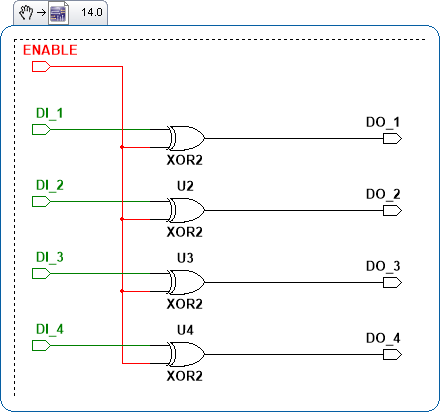
\includegraphics[width=150pt]{4bit_inverter.png}}
  \label{fig_4bit_inverter}
\end{figure}

\subsubsection{Addisjonskrets}
Å addere to binære tall er ikke nødvendigvis en triviell sak. Så for å lage en krets som utfører addisjonen er det lurt å isolere bittene og se på dem hver for seg. Binær addisjon med 1-bits tall er relativt rett frem, og er derfor mye enklere å implementere som en krets.

\paragraph{Halvadderer} 
Ved addisjon av to 1-bits tall $A$ og $B$ er det to resultater som må regnes ut og ''lagres''; delsummen $S_n$ og mente ut $C_{n+1}$. Sammenhengen mellom input og output er vist i Tabell \ref{tbl_HalfAdd}, ligning \ref{eq_sumHA} og \ref{eq_menteHA}, og Figur \ref{fig_HalfAdd} viser hvordan kretsen realiseres. 

\begin{align}
  S_n &= A_n \oplus B_n \label{eq_sumHA}\\
  C_{n+1} &= A_n B_n \label{eq_menteHA}
\end{align}

{\centering
\begin{minipage}{0.45\textwidth}
  \centering
  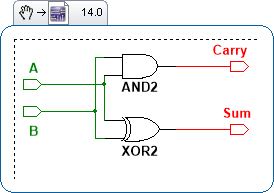
\includegraphics[width=0.9\textwidth]{halfadder.png}
  \captionof{figure}{Kretsskjema for halvadderer}
  \label{fig_HalfAdd}
\end{minipage}
\begin{minipage}{0.45\textwidth}
  \centering
  \captionof{table}{Sannhetstabell for halvadderer}
  \label{tbl_HalfAdd}
  \begin{tabular}{|ll||ll|}
        \hline
        $A_n$ & $B_n$ & $S_n$ & $C_{n+1}$ \\ 	\hline
        0 & 0 & 0 & 0 \\
        0 & 1 & 1 & 0 \\
        1 & 0 & 1 & 0 \\
        1 & 1 & 0 & 1 \\ \hline
  \end{tabular}
\end{minipage}
\endgraf\bigskip
}




\paragraph{''Ripple Carry''-adderer}
En "Ripple Carry"-adderer er en addisjonskrets egentlig bestående av fulladdere. Ved å seriekoble fulladdere slik at menteinngangene går inn i hverandre (se Figur \ref{fig_RiplFull}) har mente mulighet til å forplante seg gjennom alle fulladderene. Den er på sin mest generelle form altså istand til addere hvilke som helst binære tall av hvilke som helst størrelse, gitt at man har nok fulladdere i kretsen. Figur \ref{fig_RiplFull} viser en fire bits versjon. 

\begin{figure}
  \caption{4-bits ''Ripple Carry''-adderer kretsskjema}
  \label{fig_RiplFull}
  \centerline{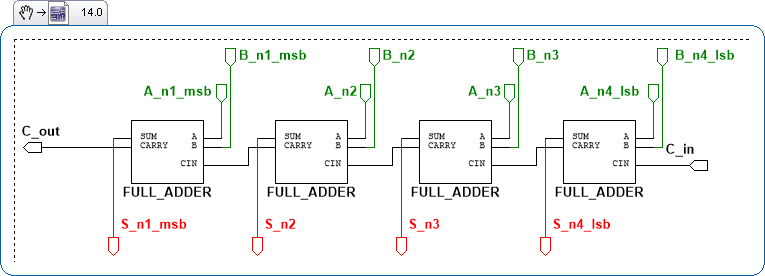
\includegraphics[width=400pt]{4bit_ripplecarry.png}}
\end{figure}

I vedlegg \ref{append_addisjon} står det mer om fulladdere, som er halvaddere med mente$inngang$, men det eneste man trenger å vite er at alle inngangene i fulladderen er likeverdige så å fjerne menteinngangssignalet $C_n$ vil være ekvivalent med å fjerne $B_n$. Tabell \ref{tbl_HalfAdd} gjelder altså også hvis inngangene er $A_n$ og $C_n$. 

\paragraph{''Adder med 1''-krets}
En av funksjonene absoluttverdikretsen må kunne utføre er å addere et tall med 1 på et ENABLE signal. For å gjøre dette skal en simplifisert ''Ripple Carry''-adderer brukes. Å addere med 1 i 4-bits binærtall vil si å addere med $0001_2$. En ''Ripple Carry''-adderer ville fint klart denne addisjonen, men det ville vært overflødig fordi det kun er det minst signifikante bittet som endres, og alle andre er 0 hele tiden. Det er meningsløst å inkludere flere innganger i kretsen som alltid adderer med 0, derfor erstattes fulladderene med halvaddere. Figur \ref{fig_riplPluss1} viser kretsskjema for dette. ENABLE signalet kobles inn i halvadderen til LSB, slik at når ENABLE er 1 vil kretsen addere med 1, og ellers vil den addere med 0. 

\begin{figure}[h]
  \caption{4-bits ''Adder med 1''-kretsskjema}
  \label{fig_riplPluss1}
  \centerline{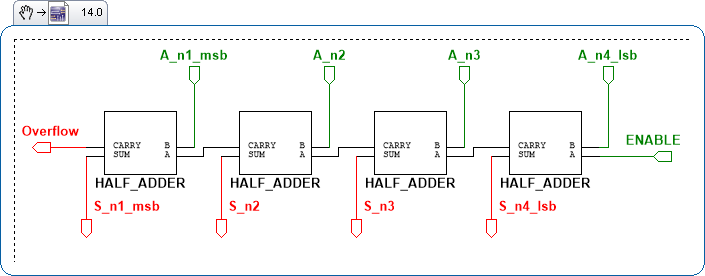
\includegraphics[width=500pt]{4bit_pluss1.png}}
\end{figure}

Merk at det også er lagt inn en overflyt indikator i Figur \ref{fig_riplPluss1}. Fordi kretsen har et veldig begrenset antall bit er overflyt en reell mulighet. Hvis inngangsignalet er $1111_2$ og ENABLE blir aktivert vil svaret bli $1 \space 0000_2$, men siden svaret er begrenset til fire bit vil det fremste bittet fjernes og resultatet blir $0000_2$. Overflyt indikatoren er der for å indikere at denne feilen har skjedd. 

\subsubsection{Absoluttverdikrets}
Fra avsnitt \ref{sec_2komp} om 2's komplement har vi at 2's komplementoperasjonen krever en invertering og en addisjon-med-1. En absoluttverdikrets må derfor kunne utføre disse operasjonene. Den må også gjenkjenne når den får et negativt tall fordi positive tall skal sendes uendret gjennom. Siden 2's komplement har fortegnsbit er det en enkel sak å kjenne igjen negative tall. Hvis MSB er 1 skal både invertering og addisjon-med-1 utføres og hvis MSB er null skal ingen av operasjonene utføres. Hvis vi setter MSB=ENABLE så vil kretsen "skru seg av og på" ved riktige tidspunkter. 
Oppkoblingen av denne kretsen er vist i Figur \ref{fig_abstractFull}. 

\begin{figure}[h]
  \caption{4-bits Absoluttverdikrets}
  \label{fig_abstractFull}
  \centerline{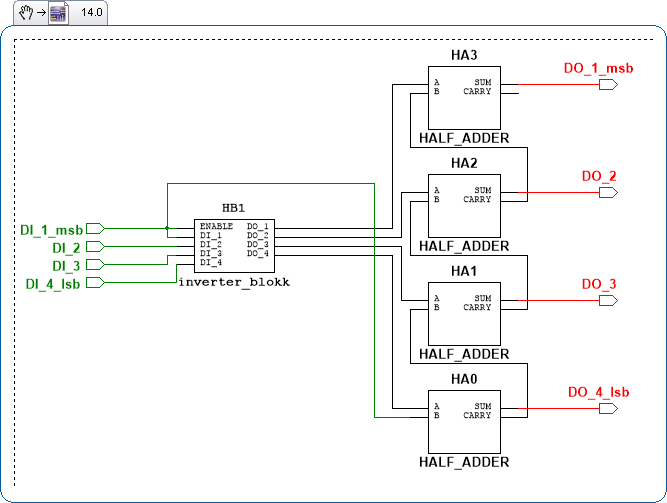
\includegraphics[width=300pt]{4bit_absoluttverdikrets_abstract.png}}
\end{figure}



\subsection{Forsinkelser}
\subsubsection{Kritisk sti}
I større kretser vil det alltid være flere veier et signal kan bevege seg gjennom på. Kritisk sti til en krets er den veien gjennom kretsen som tar lengst tid. Det er den veien som passerer flest transistorer og i enkle kretser vil det ofte være den veien som har flest logiske porter. 
I Figur \ref{fig_kritisk} er absoluttverdikretsens kritiske sti uthevet i rødt. Stien har 2 XOR porter og 3 AND porter.  

\begin{figure}[h]
  \caption{4-bits Kritisk sti i absoluttverdikrets}
  \label{fig_kritisk}
  \centerline{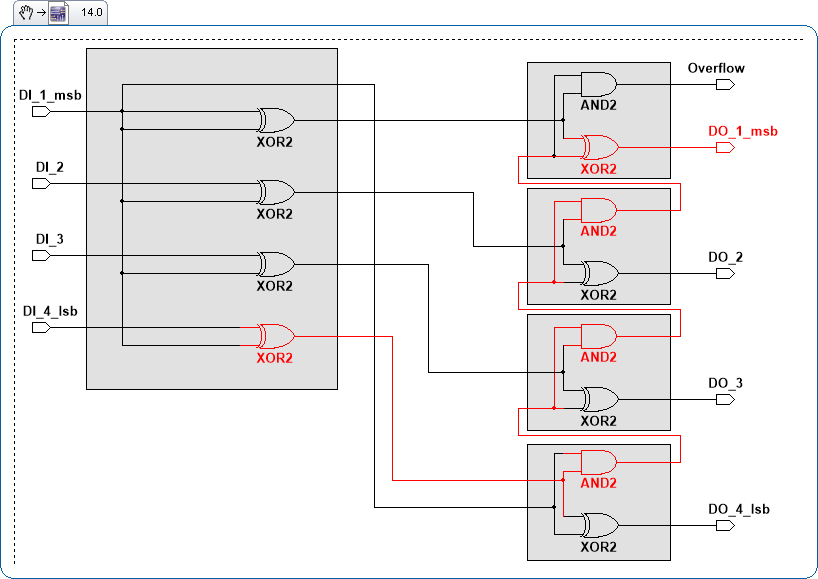
\includegraphics[width=300pt]{kritisk_sti.png}}
\end{figure}

\subsubsection{Forplantingsforsinkelse}
Forplantingsforsinkelsen til en krets er et mål på den tiden det tar for et inngangssignal å bevege seg gjennom kretsen og bli til et (stabilt) output signal. Den er definert som tiden fra inngangssignalet har steget/falt halvveis til stasjonæverdien, til utgangssignalet har steget/falt halvveis til stasjonærverdien sin. Større kretser vil logisk nok ha lengere forsinkelser, og grunnen til det er at forplantingsforsinkelsen har direkte sammenheng med antall transistorer som signalet må gå gjennom. Vi snakker ofte om forplantingsforsinkelse ift. kritisk sti, fordi da ser vi på "worst case" scenarioet hvor kretsen trenger lengst tid på å utføre kalkulasjonen. 
Å regne ut forplantingsforinkelse er en ganske rett frem prosess siden alle portkretser har en tilhørende forplantingsforsinkelse, og når man har flere porter i serie er det bare å finne summen av alle forsinkelsene. 
Absoluttverdikretsens kritiske sti er uthevet i figur \ref{fig_kritisk}, og ser der at 2 XOR porter og 3 AND porter. 

\subsubsection{Stige-/falltid}
Stige- /falltid er et mål responsen til kretsen. Stigetiden er den tiden signalet på å stige fra 10 \% til 90 \% av sin endelige verdi. Falltid er det samme bare reversert, altså tiden det tar for signalet å falle fra 90 \% til 10 \% av sin endelige verdi \cite{digtekbok}. 

\subsubsection{Maksimal Klokkefrekvens}
Maksimal klokkefrekvens er det som avgjør hvor ofte en krets kan bli oppdatert med nye inputsignaler og fremdeles gi et fornuftig outputsignal. Denne frekvensen $f_{maks}$ er definert i ligning \ref{eq_maksfrekvens} \cite{labhefte}. 

\begin{equation} \label{eq_maksfrekvens}
f_{maks} = \frac{1}{tidsforsinkelse_{kritisk \space sti}}
\end{equation}

\section{Utstyrsliste}
\begin{description}
\item[Signalgenerator]{Id. nr.: CJ891410}
\item[Oscilloskop]{Id. nr.: 604-0278}
\item[Multimeter]{Id. nr.: 503-0295}
\item[Spenningskilde]{Id. nr.: FC4403}
\item[Absoluttverdikretskort]{Id. nr.: SY0210.27922-861}
\item[Veroboardsokkel]{}
\end{description}


\section{Laboratoriearbeid} \label{sec_labarb}

\paragraph{Kontroll av halvadderer}
Vi plasserte det utdelte kretskortet i veroboardsokkelen og brukte banankabler til å koble sammen nodeparene 28-16, 28-13, 27-15 og 27-14 slik at vi fikk en halvadderer som vist i figur \ref{fig_HalfAdd}. Vi sjekket om halvadderen fungerte som den skulle ved å påtrykke 7 volt spenning. Resultatet er i Tabell \ref{tbl_halfAddTest} og det stemte med resultatet fra forarbeidet som er i Tabell \ref{tbl_HalfAdd}. 

\begin{table}[h]
\centering
\caption{Kontroll av halvadder}
\label{tbl_halfAddTest}
\begin{tabular}{|l|l||l|l|}
\hline
A, port 28 & B, port 27 & Carry & Sum \\ \hline
0          & 0          & 0     & 0   \\
0          & 1          & 0     & 1   \\
1          & 0          & 0     & 1   \\
1          & 1          & 1     & 0   \\ \hline
\end{tabular}
\end{table}

\paragraph{Absoluttverdikrets}
Så koblet vi opp absoluttverdikrets med banankabler slik at skulle få en krets tilsvarende den i figur \ref{fig_abstractFull}. Kretsens kortslutningsbøyler ble fjernet og vi sjekket om denne kretsen fungerte som den skulle ved å påtrykke 7 volt spenning. Kretsen gav riktige verdier, som var samme som i tabell \ref{tbl_absvalue}. 

\paragraph{Måling av forplantingsforsinkelse}
Fulgte prosedyren for probesjekk/probekalibrering C.6.1 i labheftet \cite{labhefte} for å sette opp proben for måling. Vi koblet sammen signalgeneratoren og oscilloskopet med BNC-BNC kabel, og brukte oscilloskopet til å stille inn signalgeneratoren til firkantpuls med frekvens 100kHz og amplitude $2,5$ V  og et DC-signal på $2,5$ V. Det vil si at signalet varierte mellom $0$ og $5$ V. Skjermdumpen fra dette er vist i figur \ref{plot_square}.

\begin{figure}[h]
  \caption{Firkantpuls}
  \label{plot_square}
  \centerline{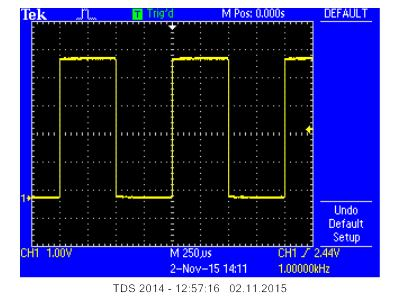
\includegraphics[width=\textwidth]{osc_square.jpg}}
\end{figure}

Vi koblet signalgeneratoren til starten av kritisk sti for å måle forplantningsforsinkelsen gjennom absoluttverdikretsen. Deretter målte vi forplantningsforsinkelsen gjennom kretsen ved å plassere proben i den andre enden av kritisk sti. I figur \ref{fig_abstractFull} svarer dette til sum-utgangen til HA3 øverst til høyre, som også er pinne U3.11 Figur 4-11 side 53 i labheftet \cite{labhefte}. 
Skjermdumpen fra oscilloskopmålingen er vist i figur \ref{plot_kritisk}. Det gule signalet er påtrykket fra signalgeneratoren mens det blå er probemålingen ved utgangen av kritisk sti. 

\begin{figure}
  \caption{Forplantingsforsinkelse gjennom kritisk sti}
  \label{plot_kritisk}
  \centerline{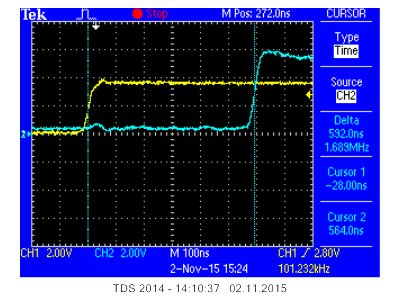
\includegraphics[width=\textwidth]{osc_kritisk.jpg}}
\end{figure}

I \ref{plot_kritisk} satte vi cursor 1 ved 50 prosent av stasjonærverdien til det inngangssignalet og cursor 2 ved 50 prosent av stasjonærverdien til utgangssignalet. Da måler vi forplantingsforsinkelsen som ble $592,0$ ns.  

\paragraph{Maksimal klokkehastighet}
Hvis vi har forplantingsforsinkelsen gjennom kritisk sti kan vi regne ut maksimal klokkehastighet med ligning \ref{eq_maksfrekvens}. 




\section{Diskusjon}
\section{Kilder}
% Referanseliste
% finn ut hvordan man endrer overskriften her

\begin{thebibliography}{}


    \bibitem{digtekbok} Svarstad, K., Kjeldsberg, P. G., Svensson, P. \& Hergum. R. (eds.)  (2014) {\em Electrical Circuits and digital design, part 2}. 
    Essex: Pearson Education Limited

    \bibitem{labhefte} Svarstad, K., Yassin, Y. H., Helland, I. \& Solvang, H. (2015) {\em TFE4101 Laboratoriehefte Høst 2015}. Trondheim: NTNU Institutt for elektronikk og telekommunikasjon
\end{thebibliography}

\newpage
\pagenumbering{roman}
\section{Vedlegg} \label{sec_append}

\subsection{Boolsk algebra i kretselementer}
Denne seksjonen vil gi en elementær innføring i hvordan boolsk algebra ser ut i kretser. Vi vil kun ta for oss de elementene som ble brukt i denne labben. 
\paragraph{AND-operasjon} 
2-inngangs AND porter er porter som gir ut 1 når begge inngangssignalene er sanne. De svarer følgelig til den Boolske AND funksjonen. 


{\centering
\begin{minipage}{0.45\textwidth}
  \centering
  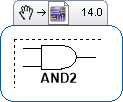
\includegraphics[width=0.9\textwidth]{port_and.png}
  \captionof{figure}{''AND'' kretssymbol}
  \label{fig_and}
\end{minipage}
\begin{minipage}{0.45\textwidth}
  \centering
  \captionof{table}{Sannhetstabell for AND}
  \label{tbl_and}
  \begin{tabular}{|ll||c|}
        \hline
        $x$ & $y$ & $xy$ \\ 	\hline
        0 & 0 & 0 \\
        0 & 1 & 0 \\
        1 & 0 & 0 \\
        1 & 1 & 1 \\ \hline
  \end{tabular}
\end{minipage}
\endgraf\bigskip
}

\paragraph{OR-operasjon}
2-inngangs OR-porter er porter som gir ut 1 når minst én av inngangene er 1. 

{\centering
\begin{minipage}{0.45\textwidth}
  \centering
  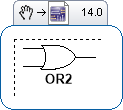
\includegraphics[width=0.9\textwidth]{port_or.png}
  \captionof{figure}{''OR'' kretssymbol}
  \label{fig_or}
\end{minipage}
\begin{minipage}{0.45\textwidth}
  \centering
  \captionof{table}{Sannhetstabell for OR}
  \label{tbl_or}
  \begin{tabular}{|ll||c|}
        \hline
        $x$ & $y$ & $x+y$ \\ 	\hline
        0 & 0 & 0 \\
        0 & 1 & 1 \\
        1 & 0 & 1 \\
        1 & 1 & 1 \\ \hline
  \end{tabular}
\end{minipage}
\endgraf\bigskip
}

\paragraph{NOT-operasjon}
NOT-porter inverterer inngangssignalet. 

{\centering
\begin{minipage}{0.45\textwidth}
  \centering
  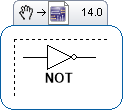
\includegraphics[width=0.9\textwidth]{port_not.png}
  \captionof{figure}{''NOT'' kretssymbol}
  \label{fig_not}
\end{minipage}
\begin{minipage}{0.45\textwidth}
  \centering
  \captionof{table}{Sannhetstabell for NOT}
  \label{tbl_not}
  \begin{tabular}{|l||l|}
        \hline
        $x$ & $\overline{x}$ \\ 	\hline
        0 & 1 \\
        1 & 0 \\ \hline
  \end{tabular}
\end{minipage}
\endgraf\bigskip
}

\paragraph{XOR-operasjon}
XOR er en litt mer avansert funksjon. Det betyr eksklusiv OR og den gir 1 når en av inngangene er 1, men 0 når begge er 1. Algebraisk kan den skrives slik:
$$ x \oplus y = x\bar{y} + \bar{x}y$$
Siden XOR-operasjonen er mye brukt i kretser har den et eget symbol. I kretsskissen i figur \ref{fig_xor} viser kretssymbolet og figur \ref{fig_xorbuild} viser innsiden av dette symbolet som en sammensetning av OR-, AND- og NOT-porter. Merk at virkelige XOR-porter kan se litt annerledes ut på innsiden, men poenget er å vise at kompleksiteten til XOR-operasjonen gjør at selve kretselementet blir vesentlig mer innviklet. 

{\centering
\begin{minipage}{0.30\textwidth}
  \centering
  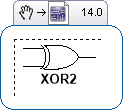
\includegraphics[width=0.9\textwidth]{port_xor.png}
  \captionof{figure}{''XOR'' kretssymbol}
  \label{fig_xor}
\end{minipage}
\begin{minipage}{0.30\textwidth}
  \centering
  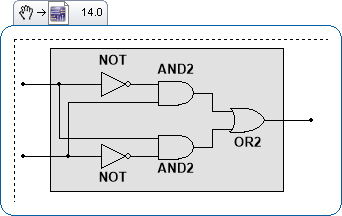
\includegraphics[width=0.9\textwidth]{port_xorbuild.png}
  \captionof{figure}{Oppbygning av XOR}
  \label{fig_xorbuild}
\end{minipage}
\begin{minipage}{0.30\textwidth}
  \centering
  \captionof{table}{Sannhetstabell for XOR}
  \label{tbl_xor}
  \begin{tabular}{|ll||c|}
        \hline
        $x$ & $y$ & $x \oplus y$ \\ \hline
        0 & 0 & 0 \\
        0 & 1 & 1 \\
        1 & 0 & 1 \\
        1 & 1 & 0 \\ \hline
  \end{tabular}
\end{minipage}
\endgraf\bigskip
}

\paragraph{NAND-operasjon}
Dette er den inverteringen av en AND-operasjon og implementeres ved hjelp av en AND- og (en etterfølgende) NOT-port. 

{\centering
\begin{minipage}{0.45\textwidth}
  \centering
  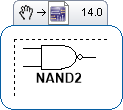
\includegraphics[width=0.9\textwidth]{port_nand.png}
  \captionof{figure}{''NAND'' kretssymbol}
  \label{fig_nand}
\end{minipage}
\begin{minipage}{0.45\textwidth}
  \centering
  \captionof{table}{Sannhetstabell for NAND}
  \label{tbl_nand}
  \begin{tabular}{|l|l||l|}
        \hline
        $x$ & $y$ 	& $\overline{xy}$ \\ 	\hline
        0 	& 0 	& 1\\
        0 	& 1 	& 1\\
        1 	& 0 	& 1\\
        1 	& 1 	& 0\\ \hline
  \end{tabular}
\end{minipage}
\endgraf\bigskip
}


\subsection{Mer om addisjonskretser} \label{append_addisjon}
\paragraph{Full-adderer}
For å lage en fullverdig addisjonskrets trenger vi en 1-bit adderer som kan ta hensyn til mente inn. Så i tillegg til inngangsignalene $A_n$ og $B_n$ må den ha et tredje inngangssignal $C_n$, som tilsvarer mente inn. Sammenhengen mellom signalene er her gitt av sannhetstabellen Tabell \ref{tbl_FullAdd} og ligning \ref{eq_sumFA} og \ref{eq_menteFA}. 

\begin{align}
S_n &= A_n \oplus B_n \oplus C_n \label{eq_sumFA}\\
C_{n+1} &= A_n B_n + A_n C_n + B_n C_n \label{eq_menteFA}
\end{align}

\begin{table}[h]
      \centering
        \caption{Sannhetstabell for fulladderer}
        \label{tbl_FullAdd}
        \begin{tabular}{|lll||ll|}
        \hline
        $A_n$ & $B_n$ & $C_n$ & $S_n$ & $C_{n+1}$ \\ \hline
        0 & 0 & 0 & 0 & 0\\
        0 & 0 & 1 & 1 & 0\\
        0 & 1 & 0 & 1 & 0\\
        0 & 1 & 1 & 0 & 1\\
        1 & 0 & 0 & 1 & 0\\
        1 & 0 & 1 & 0 & 1\\
        1 & 1 & 0 & 0 & 1\\
        1 & 1 & 1 & 1 & 1\\ \hline
      \end{tabular}
\end{table}

\subsection{Datablader (utdrag)}
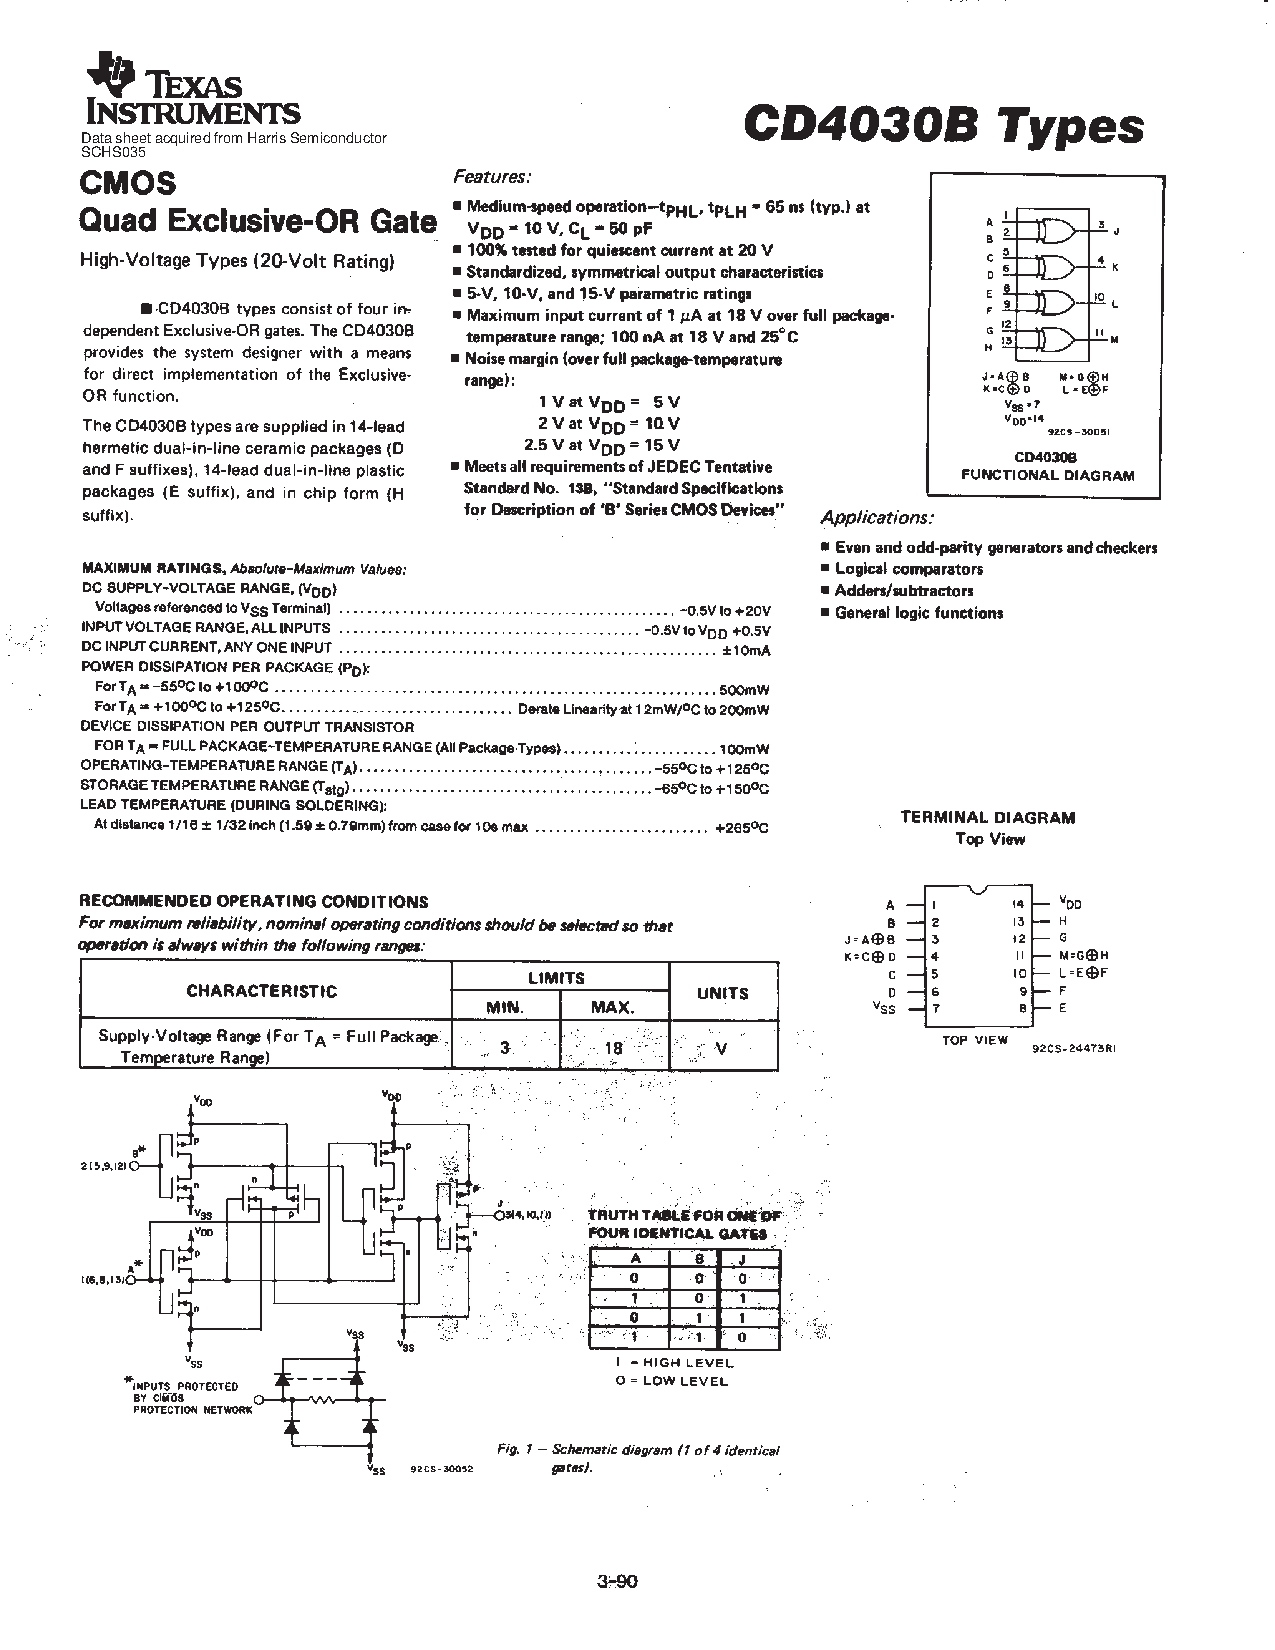
\includepdf[pages={1-3}]{cd4030.pdf}
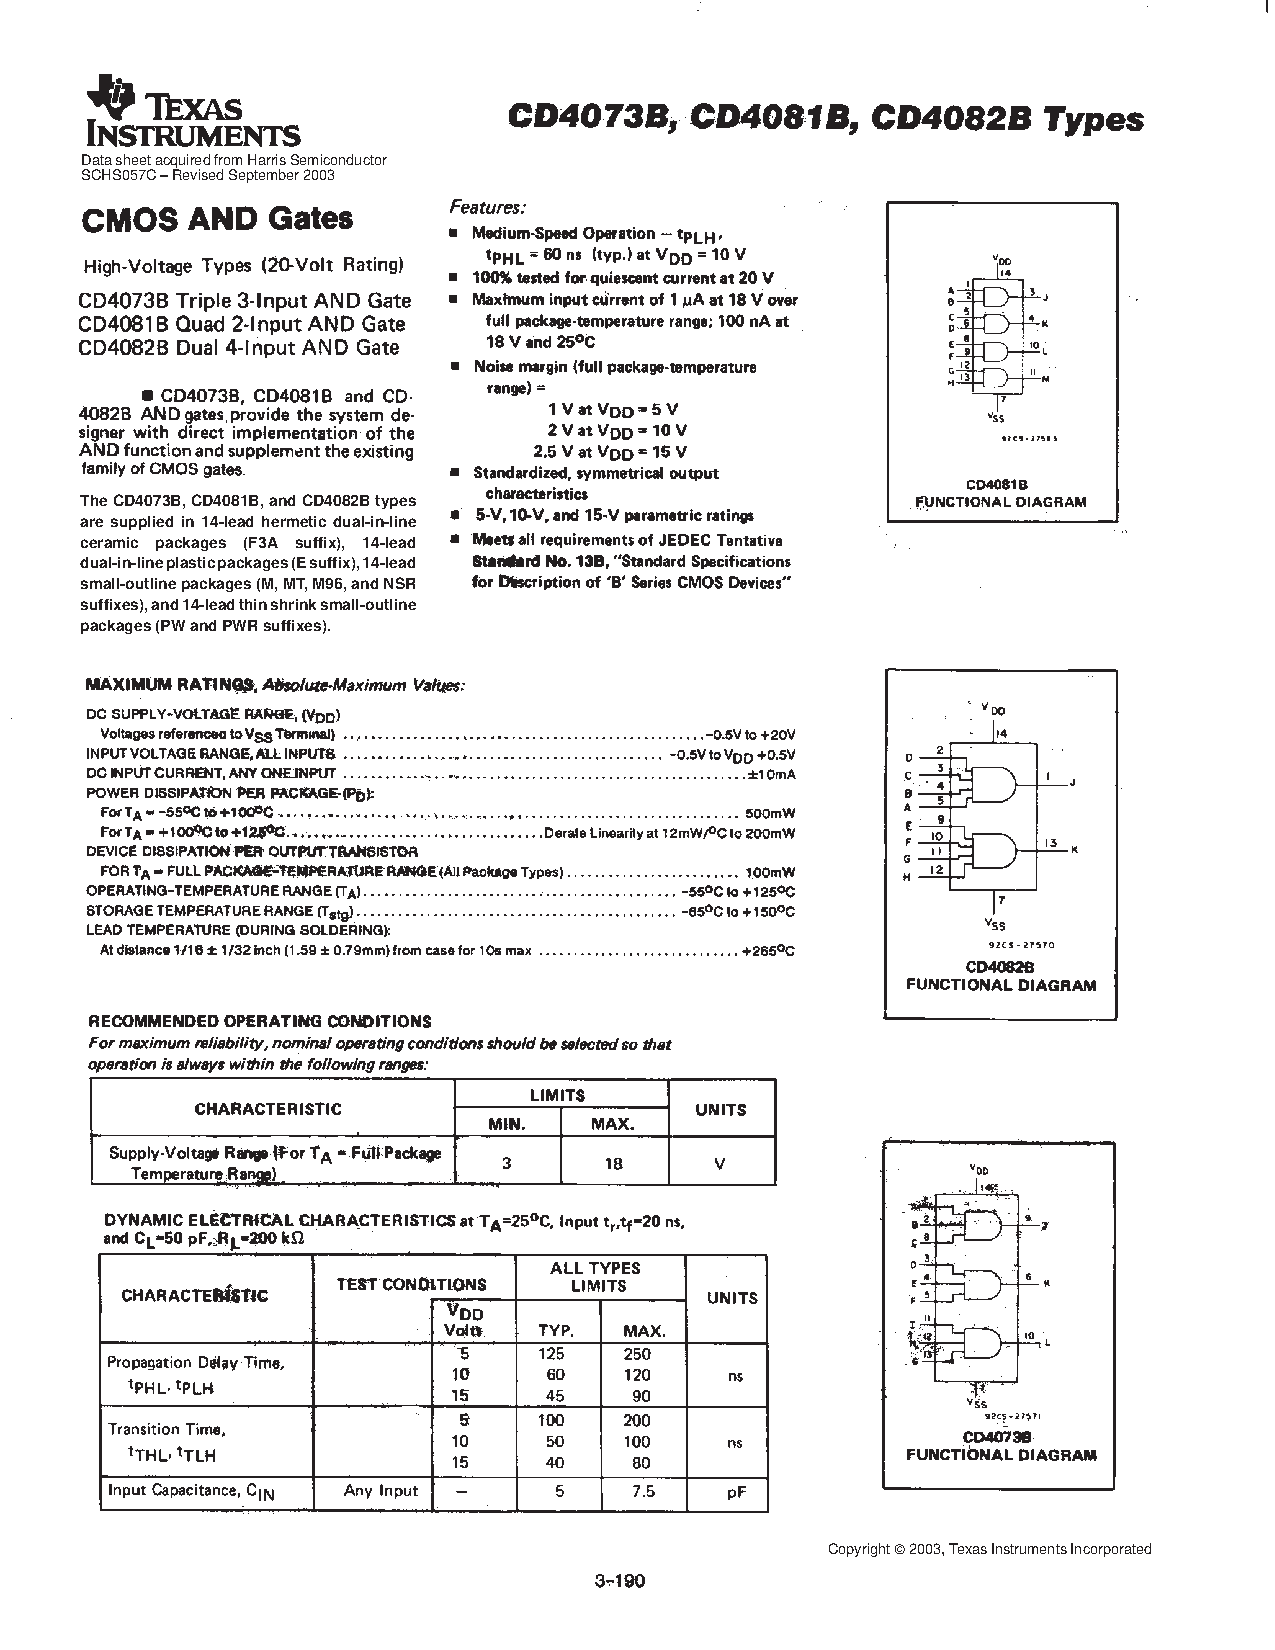
\includepdf[pages={1-3}]{cd4081b.pdf}



\end{document}
